\clearpage\section{实验结果与分析}

\FloatBarrier\subsection{总体结果}

各模型的总体结果、类指标分别见表~\ref{tab:4-1}、表~\ref{tab:4-2}，单次结果的区间见图~\ref{fig:4-1}。多种子模型报告 3 次运行的均值与标准差；置信区间为种子 42 运行的 Bootstrap 95\% 置信区间。

\begin{table}[htbp]
\centering
\begin{minipage}{\textwidth}
\setlength{\tabcolsep}{3pt}
\renewcommand{\arraystretch}{1.16}
\setstretch{1.0}\fontsize{10.5}{13.5}\selectfont
\caption{总体分类结果与单次运行区间}\label{tab:4-1}
\begin{tabular}{>{\raggedright\arraybackslash}p{\dimexpr 0.300000\linewidth-3.000000\tabcolsep\relax}>{\raggedright\arraybackslash}p{\dimexpr 0.070000\linewidth-0.700000\tabcolsep\relax}>{\raggedright\arraybackslash}p{\dimexpr 0.200000\linewidth-2.000000\tabcolsep\relax}>{\raggedright\arraybackslash}p{\dimexpr 0.200000\linewidth-2.000000\tabcolsep\relax}>{\raggedright\arraybackslash}p{\dimexpr 0.230000\linewidth-2.300000\tabcolsep\relax}}
\toprule
\textbf{模型} & \textbf{次数} & \textbf{准确率} & \textbf{Macro-\allowbreak{}F1} & \textbf{单次 F1 的 95\% CI} \\
\midrule
TF-\allowbreak{}IDF + 逻辑回归 & 1 & 0.734 & 0.702 & [0.679, 0.725] \\
TF-\allowbreak{}IDF + SVM & 1 & 0.735 & 0.693 & [0.670, 0.716] \\
BERT & 3 & 0.785 $\pm$ 0.009 & 0.758 $\pm$ 0.010 & [0.731, 0.774] \\
RoBERTa & 3 & 0.802 $\pm$ 0.005 & 0.778 $\pm$ 0.005 & [0.759, 0.801] \\
Qwen3-\allowbreak{}8B 零样本 & 1 & 0.671 & 0.644 & [0.620, 0.666] \\
Qwen2.5-\allowbreak{}7B 零样本 & 1 & 0.702 & 0.666 & [0.642, 0.688] \\
GLM-\allowbreak{}4-\allowbreak{}9B 零样本 & 1 & 0.682 & 0.661 & [0.638, 0.684] \\
Qwen3-\allowbreak{}8B 少样本（每类 3 例） & 1 & 0.713 & 0.696 & [0.674, 0.718] \\
Qwen2.5-\allowbreak{}7B 少样本（每类 3 例） & 1 & 0.712 & 0.690 & [0.667, 0.711] \\
GLM-\allowbreak{}4-\allowbreak{}9B 少样本（每类 3 例） & 1 & 0.645 & 0.627 & [0.604, 0.651] \\
\textbf{Qwen3-\allowbreak{}8B + LoRA} & 3 & 0.821 $\pm$ 0.001 & 0.801 $\pm$ 0.002 & [0.779, 0.820] \\
\textbf{Qwen2.5-\allowbreak{}7B + LoRA} & 3 & 0.826 $\pm$ 0.007 & \textbf{0.807 $\pm$ 0.007} & [0.778, 0.818] \\
\textbf{GLM-\allowbreak{}4-\allowbreak{}9B + LoRA} & 3 & 0.818 $\pm$ 0.004 & 0.798 $\pm$ 0.004 & [0.778, 0.818] \\
\bottomrule\end{tabular}
\par\vspace{3pt}{\fontsize{10}{12.5}\selectfont 注：均值$\pm$标准差基于三个种子；95\% 区间仅对应种子 42（或单次运行），采用 B=2000 的测试样本 Bootstrap，不是三种子均值的区间。\par}
\end{minipage}
\end{table}

\begin{table}[htbp]
\centering
\begin{minipage}{\textwidth}
\setlength{\tabcolsep}{3pt}
\renewcommand{\arraystretch}{1.16}
\setstretch{1.0}\fontsize{10.5}{13.5}\selectfont
\caption{各类别 F1}\label{tab:4-2}
\begin{tabular}{>{\raggedright\arraybackslash}p{\dimexpr 0.400000\linewidth-3.200000\tabcolsep\relax}>{\raggedright\arraybackslash}p{\dimexpr 0.200000\linewidth-1.600000\tabcolsep\relax}>{\raggedright\arraybackslash}p{\dimexpr 0.200000\linewidth-1.600000\tabcolsep\relax}>{\raggedright\arraybackslash}p{\dimexpr 0.200000\linewidth-1.600000\tabcolsep\relax}}
\toprule
\textbf{模型} & \textbf{消极 F1} & \textbf{中性 F1} & \textbf{积极 F1} \\
\midrule
TF-\allowbreak{}IDF + 逻辑回归 & 0.735 & 0.550 & 0.820 \\
TF-\allowbreak{}IDF + SVM & 0.740 & 0.526 & 0.813 \\
BERT & 0.793 & 0.630 & 0.851 \\
RoBERTa & 0.813 & 0.660 & 0.862 \\
Qwen3-\allowbreak{}8B 零样本 & 0.701 & 0.474 & 0.758 \\
Qwen2.5-\allowbreak{}7B 零样本 & 0.720 & 0.482 & 0.796 \\
GLM-\allowbreak{}4-\allowbreak{}9B 零样本 & 0.712 & 0.515 & 0.757 \\
Qwen3-\allowbreak{}8B 少样本（每类 3 例） & 0.755 & 0.546 & 0.788 \\
Qwen2.5-\allowbreak{}7B 少样本（每类 3 例） & 0.752 & 0.532 & 0.786 \\
GLM-\allowbreak{}4-\allowbreak{}9B 少样本（每类 3 例） & 0.702 & 0.471 & 0.708 \\
\textbf{Qwen3-\allowbreak{}8B + LoRA} & 0.848 & 0.686 & 0.871 \\
\textbf{Qwen2.5-\allowbreak{}7B + LoRA} & 0.839 & \textbf{0.707} & 0.877 \\
\textbf{GLM-\allowbreak{}4-\allowbreak{}9B + LoRA} & 0.833 & 0.689 & 0.872 \\
\bottomrule\end{tabular}
\par\vspace{3pt}{\fontsize{10}{12.5}\selectfont 注：多种子模型为三次类 F1 的均值，其他模型为单次结果；与后文种子 42 错误分析分开解读。\par}
\end{minipage}
\end{table}

\begin{figure}[htbp]\centering
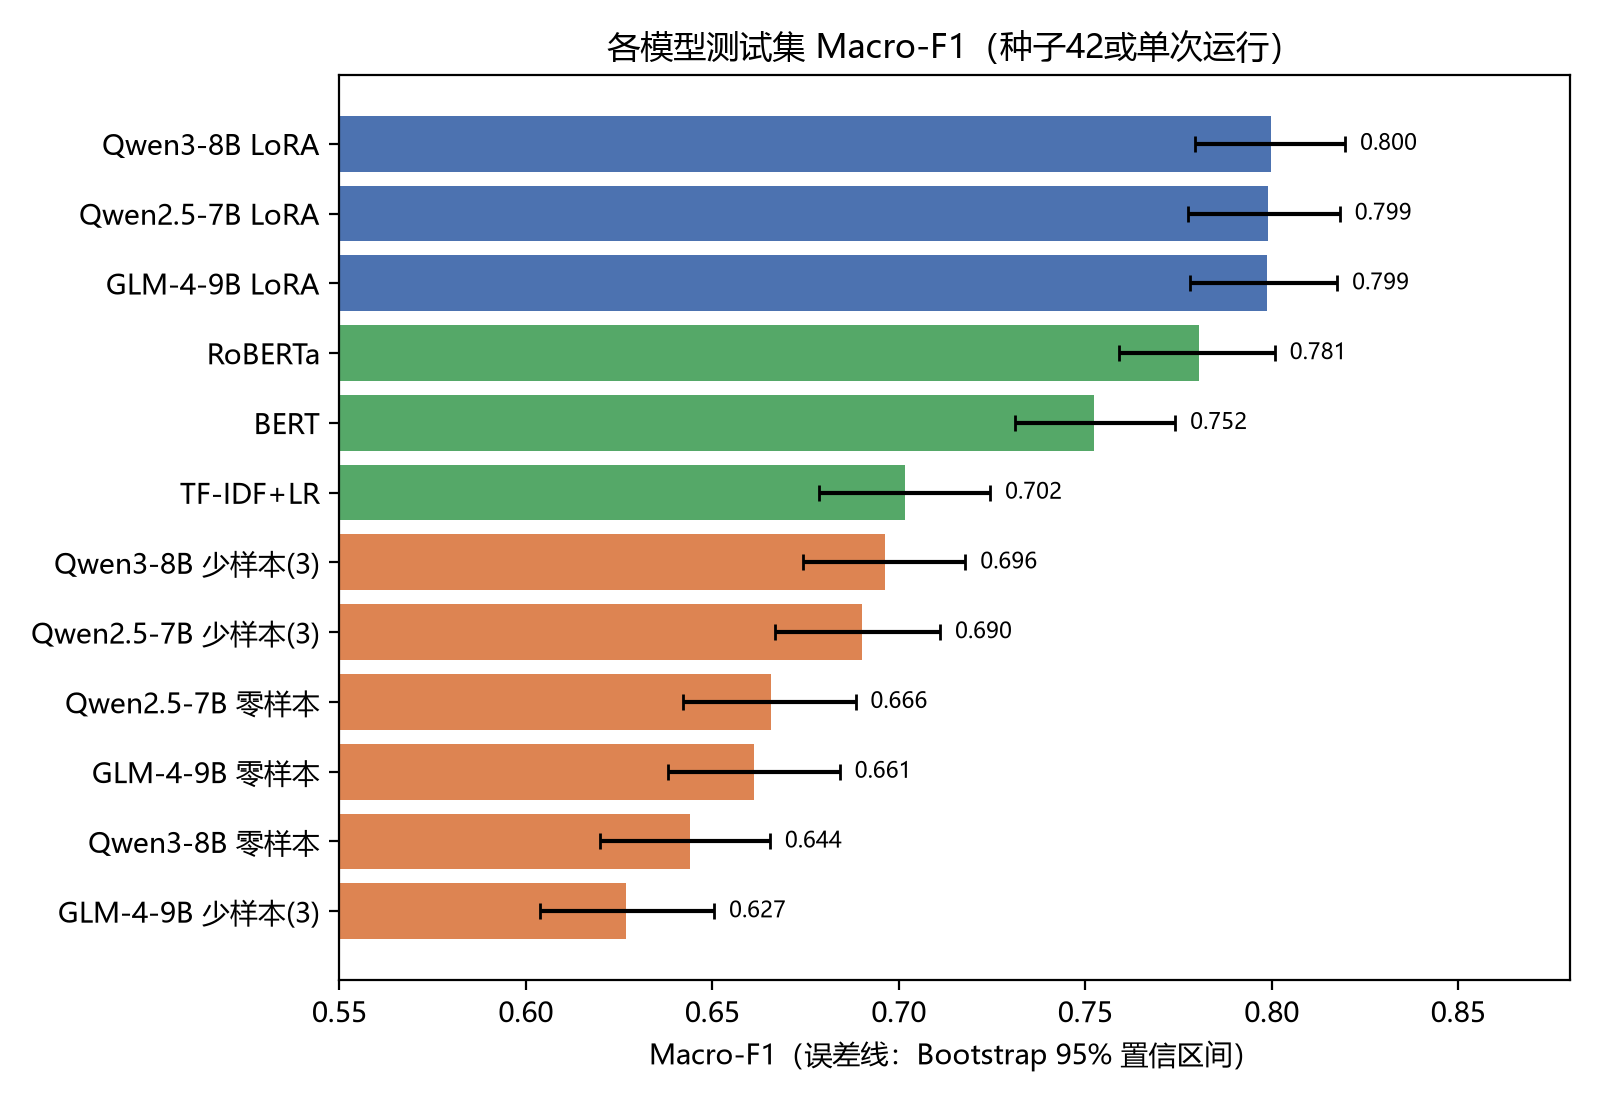
\includegraphics[width=\linewidth,height=0.80\textheight,keepaspectratio]{figures/fig_model_comparison.png}
\caption{各模型种子 42 或单次运行的 Macro-\allowbreak{}F1（柱高与 Bootstrap 95\% 区间对应同一次运行）}\label{fig:4-1}\end{figure}

综合表~\ref{tab:4-1} 与表~\ref{tab:4-2} 可以得出以下几点：

第一，LoRA 微调后的三个大模型取得了最好的效果，Macro-F1 在 0.798～0.807 之间，准确率在 81.8\%～82.6\% 之间。其中 Qwen2.5-7B 的平均 Macro-F1 最高（0.807），但三个大模型之间的差距不超过 0.01。

第二，不经微调的大模型表现较差。三个模型零样本的 Macro-F1 只有 0.644～0.666，甚至低于最简单的 TF-IDF + 逻辑回归（0.702）。这与 DISC-FinLLM\cite{ref33} 等研究报告的通用大模型在 FinFE 上准确率约为 60\%～69\% 的结论一致，与通用提示难以直接匹配本任务标签分布的解释相容，但并不能单凭分数定位为模型缺少某类知识。

第三，提供示例的作用有限且不稳定。每类给出 3 个示例时，Qwen3-8B 的 Macro-F1 从 0.644 提高到 0.696，Qwen2.5-7B 从 0.666 提高到 0.690，而 GLM-4-9B 反而从 0.661 下降到 0.627。每类只给 1 个示例时，GLM-4-9B 同样下降（0.630），Qwen2.5-7B 基本不变（0.666）。在当前固定提示和示例抽样下，少样本收益因模型而异；没有重复抽取示例，不能将这一结果外推为提示方法普遍不可靠。

第四，所有模型在中性类上的 F1 都明显低于另外两类。即使是表现最好的模型，中性类 F1 也只有 0.707，比积极类低约 17 个百分点。结合 3.3 节的描述性统计，中性评论多为提问或客观陈述，与带有轻微情绪的消极、积极评论边界模糊；数据清洗中发现的 228 条跨文件标签不一致样本也说明，人工标注在这些样本上同样存在分歧。

\FloatBarrier\subsection{显著性检验}

\subsubsection{McNemar 检验}

表~\ref{tab:4-3} 列出了 TF-IDF + 逻辑回归、RoBERTa 和三个 LoRA 大模型（均取种子 42 的运行）两两之间的 McNemar 检验结果，p 值经 Holm 方法校正。

\begin{table}[htbp]
\centering
\begin{minipage}{\textwidth}
\setlength{\tabcolsep}{3pt}
\renewcommand{\arraystretch}{1.16}
\setstretch{1.0}\fontsize{10.5}{13.5}\selectfont
\caption{McNemar 检验结果（Holm 校正）}\label{tab:4-3}
\begin{tabular}{>{\raggedright\arraybackslash}p{\dimexpr 0.200000\linewidth-2.800000\tabcolsep\relax}>{\raggedright\arraybackslash}p{\dimexpr 0.200000\linewidth-2.800000\tabcolsep\relax}>{\raggedright\arraybackslash}p{\dimexpr 0.120000\linewidth-1.680000\tabcolsep\relax}>{\raggedright\arraybackslash}p{\dimexpr 0.120000\linewidth-1.680000\tabcolsep\relax}>{\raggedright\arraybackslash}p{\dimexpr 0.120000\linewidth-1.680000\tabcolsep\relax}>{\raggedright\arraybackslash}p{\dimexpr 0.120000\linewidth-1.680000\tabcolsep\relax}>{\raggedright\arraybackslash}p{\dimexpr 0.120000\linewidth-1.680000\tabcolsep\relax}}
\toprule
\textbf{模型 A} & \textbf{模型 B} & \textbf{A 对 B 错} & \textbf{A 错 B 对} & \textbf{$\chi^{2}$} & \textbf{原始 p 值} & \textbf{校正后 p 值} \\
\midrule
TF-\allowbreak{}IDF+LR & RoBERTa & 101 & 223 & 45.19 & 1.8$\times$10$^{-11}$ & 1.3$\times$10$^{-10}$ \\
TF-\allowbreak{}IDF+LR & Qwen3-\allowbreak{}8B LoRA & 109 & 257 & 59.04 & 1.5$\times$10$^{-14}$ & 1.5$\times$10$^{-13}$ \\
TF-\allowbreak{}IDF+LR & Qwen2.5-\allowbreak{}7B LoRA & 112 & 255 & 54.94 & 1.2$\times$10$^{-13}$ & 1.1$\times$10$^{-12}$ \\
TF-\allowbreak{}IDF+LR & GLM-\allowbreak{}4-\allowbreak{}9B LoRA & 118 & 263 & 54.43 & 1.6$\times$10$^{-13}$ & 1.3$\times$10$^{-12}$ \\
RoBERTa & Qwen3-\allowbreak{}8B LoRA & 97 & 123 & 2.84 & 0.092 & 0.551 \\
RoBERTa & Qwen2.5-\allowbreak{}7B LoRA & 83 & 104 & 2.14 & 0.144 & 0.695 \\
RoBERTa & GLM-\allowbreak{}4-\allowbreak{}9B LoRA & 99 & 122 & 2.19 & 0.139 & 0.695 \\
Qwen3-\allowbreak{}8B LoRA & Qwen2.5-\allowbreak{}7B LoRA & 82 & 77 & 0.10 & 0.751 & 1.000 \\
Qwen3-\allowbreak{}8B LoRA & GLM-\allowbreak{}4-\allowbreak{}9B LoRA & 85 & 82 & 0.02 & 0.877 & 1.000 \\
Qwen2.5-\allowbreak{}7B LoRA & GLM-\allowbreak{}4-\allowbreak{}9B LoRA & 87 & 89 & 0.01 & 0.940 & 1.000 \\
\bottomrule\end{tabular}
\end{minipage}
\end{table}

结果显示：RoBERTa 和三个大模型均极显著优于 TF-IDF 基线；三个大模型之间差异很小，两个模型判断不一致的样本中，双方各对一半左右，校正后 p 值均为 1；大模型与 RoBERTa 相比，虽然``大模型对、RoBERTa 错''的样本多于反向情况（如 123 对 97），但即使不做校正也未达到 0.05 的显著性水平，校正后 p 值在 0.55～0.70 之间。

\subsubsection{配对 Bootstrap}

McNemar 检验只关注准确率。表~\ref{tab:4-4} 给出以 Macro-F1 为指标的配对 Bootstrap 结果（B = 50000，种子 42 的模型预测）。表中展示六对主要比较，但多重比较家族包含五模型的全部十对，并未因展示范围而缩小。

\begin{table}[htbp]
\centering
\begin{minipage}{\textwidth}
\setlength{\tabcolsep}{3pt}
\renewcommand{\arraystretch}{1.16}
\setstretch{1.0}\fontsize{10.5}{13.5}\selectfont
\caption{配对 Bootstrap：Macro-\allowbreak{}F1 差值与区间}\label{tab:4-4}
\begin{tabular}{>{\raggedright\arraybackslash}p{\dimexpr 0.200000\linewidth-2.000000\tabcolsep\relax}>{\raggedright\arraybackslash}p{\dimexpr 0.200000\linewidth-2.000000\tabcolsep\relax}>{\raggedright\arraybackslash}p{\dimexpr 0.120000\linewidth-1.200000\tabcolsep\relax}>{\raggedright\arraybackslash}p{\dimexpr 0.240000\linewidth-2.400000\tabcolsep\relax}>{\raggedright\arraybackslash}p{\dimexpr 0.240000\linewidth-2.400000\tabcolsep\relax}}
\toprule
\textbf{模型 A} & \textbf{模型 B} & \textbf{差值（A $-$ B）} & \textbf{单比较 95\% 区间} & \textbf{Bonferroni 调整区间} \\
\midrule
RoBERTa & Qwen3-\allowbreak{}8B LoRA & -\allowbreak{}0.01929 & [-\allowbreak{}0.03885, 0.00012] & [-\allowbreak{}0.04725, 0.00892] \\
RoBERTa & Qwen2.5-\allowbreak{}7B LoRA & -\allowbreak{}0.01829 & [-\allowbreak{}0.03608, -\allowbreak{}0.00079] & [-\allowbreak{}0.04357, 0.00690] \\
RoBERTa & GLM-\allowbreak{}4-\allowbreak{}9B LoRA & -\allowbreak{}0.01816 & [-\allowbreak{}0.03785, 0.00126] & [-\allowbreak{}0.04667, 0.01032] \\
Qwen3-\allowbreak{}8B LoRA & Qwen2.5-\allowbreak{}7B LoRA & 0.00099 & [-\allowbreak{}0.01554, 0.01713] & [-\allowbreak{}0.02244, 0.02414] \\
Qwen3-\allowbreak{}8B LoRA & GLM-\allowbreak{}4-\allowbreak{}9B LoRA & 0.00112 & [-\allowbreak{}0.01570, 0.01808] & [-\allowbreak{}0.02305, 0.02547] \\
Qwen2.5-\allowbreak{}7B LoRA & GLM-\allowbreak{}4-\allowbreak{}9B LoRA & 0.00013 & [-\allowbreak{}0.01706, 0.01746] & [-\allowbreak{}0.02440, 0.02465] \\
\bottomrule\end{tabular}
\end{minipage}
\end{table}

两个 Qwen 模型和 GLM 相对 RoBERTa 的 F1 点估计均高约 1.8～1.9 个百分点。在未调整区间中，仅 Qwen2.5 的区间不包含 0；经十对比较的 Bonferroni 调整后，三个 LoRA 对 RoBERTa 的区间均包含 0。Qwen3 的未调整区间边界非常接近 0，提示结论对重抽样误差敏感，不宜用单个区间是否刚好跨 0 强调``边缘显著''。三个 LoRA 模型之间的调整区间也均包含 0，未检出差异不等于证明效果相同。

\subsubsection{多种子方差分析}

表~\ref{tab:4-5} 为五个多种子模型的 Macro-F1 方差分析结果。

\begin{table}[htbp]
\centering
\begin{minipage}{\textwidth}
\setlength{\tabcolsep}{3pt}
\renewcommand{\arraystretch}{1.16}
\setstretch{1.0}\fontsize{10.5}{13.5}\selectfont
\caption{多种子 Macro-\allowbreak{}F1 方差分析}\label{tab:4-5}
\begin{tabular}{>{\raggedright\arraybackslash}p{\dimexpr 0.333333\linewidth-2.000000\tabcolsep\relax}>{\raggedright\arraybackslash}p{\dimexpr 0.333333\linewidth-2.000000\tabcolsep\relax}>{\raggedright\arraybackslash}p{\dimexpr 0.333333\linewidth-2.000000\tabcolsep\relax}}
\toprule
\textbf{检验} & \textbf{统计量} & \textbf{p 值} \\
\midrule
Levene 方差齐性检验 & W = 0.262 & 0.896 \\
单因素方差分析（5 组） & F = 31.87 & 1.1$\times$10$^{-5}$ \\
Welch 方差分析（5 组） & F = 19.84 & 0.004 \\
单因素方差分析（仅三个 LoRA 大模型） & F = 2.78 & 0.140 \\
\bottomrule\end{tabular}
\end{minipage}
\end{table}

Levene 检验未检出方差差异（p = 0.896），但每组仅 3 次，不能据此证明方差相等，单因素方差分析和 Welch 方差分析均显示五个模型的平均 Macro-F1 存在显著差异。Tukey HSD 事后比较（表~\ref{tab:4-6}）表明：三个 LoRA 大模型均显著优于 RoBERTa（平均高 2.0～2.9 个百分点，p \textless{} 0.03），RoBERTa 显著优于 BERT（p = 0.017），而三个大模型之间两两差异均不显著（p \textgreater{} 0.38）。

\begin{table}[htbp]
\centering
\begin{minipage}{\textwidth}
\setlength{\tabcolsep}{3pt}
\renewcommand{\arraystretch}{1.16}
\setstretch{1.0}\fontsize{10.5}{13.5}\selectfont
\caption{Tukey HSD 事后比较（均值差 = 组 2 $-$ 组 1）}\label{tab:4-6}
\begin{tabular}{>{\raggedright\arraybackslash}p{\dimexpr 0.200000\linewidth-2.000000\tabcolsep\relax}>{\raggedright\arraybackslash}p{\dimexpr 0.200000\linewidth-2.000000\tabcolsep\relax}>{\raggedright\arraybackslash}p{\dimexpr 0.120000\linewidth-1.200000\tabcolsep\relax}>{\raggedright\arraybackslash}p{\dimexpr 0.140000\linewidth-1.400000\tabcolsep\relax}>{\raggedright\arraybackslash}p{\dimexpr 0.340000\linewidth-3.400000\tabcolsep\relax}}
\toprule
\textbf{组 1} & \textbf{组 2} & \textbf{均值差} & \textbf{调整后 p 值} & \textbf{95\% 置信区间} \\
\midrule
BERT & RoBERTa & 0.020 & 0.017 & [0.004, 0.037] \\
RoBERTa & Qwen3-\allowbreak{}8B LoRA & 0.023 & 0.008 & [0.006, 0.040] \\
RoBERTa & Qwen2.5-\allowbreak{}7B LoRA & 0.029 & 0.001 & [0.012, 0.046] \\
RoBERTa & GLM-\allowbreak{}4-\allowbreak{}9B LoRA & 0.020 & 0.021 & [0.003, 0.036] \\
Qwen3-\allowbreak{}8B LoRA & Qwen2.5-\allowbreak{}7B LoRA & 0.006 & 0.754 & [$-$0.011, 0.023] \\
GLM-\allowbreak{}4-\allowbreak{}9B LoRA & Qwen3-\allowbreak{}8B LoRA & 0.003 & 0.958 & [$-$0.013, 0.020] \\
GLM-\allowbreak{}4-\allowbreak{}9B LoRA & Qwen2.5-\allowbreak{}7B LoRA & 0.010 & 0.389 & [$-$0.007, 0.026] \\
\bottomrule\end{tabular}
\end{minipage}
\end{table}

\subsubsection{检验结果的综合解读}

不同方法考察的随机性与评价指标并不相同。多种子 ANOVA 和 Tukey 比较条件于当前训练、验证和测试划分，反映有限训练重复间的差异；McNemar 与配对 Bootstrap 条件于种子 42 的训练结果，考察测试样本的配对抽样误差，且分别针对准确率和 Macro-F1。前者的显著结果不能替代后者，也不能替代面向新数据的验证。

在所考察的三个种子中，三个 LoRA 模型的 F1 点估计均高于 RoBERTa，平均差为约 2.0～2.9 个百分点；但种子 42 的 McNemar 检验和配对 Bootstrap 在各自的多重比较调整后均未检出显著优势。因此，本文将结论限定为``在本数据划分和三个训练种子中观察到一致较高的点估计''，不推广为对新样本的稳定优越性。三个 LoRA 模型之间未检出差异，也不构成等效性结论。

\FloatBarrier\subsection{校准分析}

原始概率指标与温度交叉拟合结果分别见表~\ref{tab:4-7}、表~\ref{tab:4-8}，可靠性图见图~\ref{fig:4-2}。

\begin{table}[htbp]
\centering
\begin{minipage}{\textwidth}
\setlength{\tabcolsep}{3pt}
\renewcommand{\arraystretch}{1.16}
\setstretch{1.0}\fontsize{10.5}{13.5}\selectfont
\caption{原始概率的校准指标（种子 42 或单次）}\label{tab:4-7}
\begin{tabular}{>{\raggedright\arraybackslash}p{\dimexpr 0.300000\linewidth-3.600000\tabcolsep\relax}>{\raggedright\arraybackslash}p{\dimexpr 0.140000\linewidth-1.680000\tabcolsep\relax}>{\raggedright\arraybackslash}p{\dimexpr 0.140000\linewidth-1.680000\tabcolsep\relax}>{\raggedright\arraybackslash}p{\dimexpr 0.140000\linewidth-1.680000\tabcolsep\relax}>{\raggedright\arraybackslash}p{\dimexpr 0.140000\linewidth-1.680000\tabcolsep\relax}>{\raggedright\arraybackslash}p{\dimexpr 0.140000\linewidth-1.680000\tabcolsep\relax}}
\toprule
\textbf{模型} & \textbf{平均置信度} & \textbf{准确率} & \textbf{ECE} & \textbf{Brier} & \textbf{NLL} \\
\midrule
TF-\allowbreak{}IDF+LR & 0.777 & 0.734 & 0.045 & 0.367 & 0.651 \\
RoBERTa & 0.830 & 0.806 & 0.031 & 0.276 & 0.493 \\
Qwen3-\allowbreak{}8B 零样本 & 0.964 & 0.671 & 0.294 & 0.610 & 3.330 \\
Qwen3-\allowbreak{}8B LoRA & 0.880 & 0.821 & 0.061 & 0.266 & 0.486 \\
Qwen2.5-\allowbreak{}7B LoRA & 0.852 & 0.818 & 0.035 & 0.261 & 0.474 \\
GLM-\allowbreak{}4-\allowbreak{}9B LoRA & 0.900 & 0.819 & 0.085 & 0.281 & 0.527 \\
\bottomrule\end{tabular}
\par\vspace{3pt}{\fontsize{10}{12.5}\selectfont 注：由历史六位小数概率计算，NLL 截断下限为 1e-\allowbreak{}12；零样本敏感性见本节。\par}
\end{minipage}
\end{table}

\begin{table}[htbp]
\centering
\begin{minipage}{\textwidth}
\setlength{\tabcolsep}{3pt}
\renewcommand{\arraystretch}{1.16}
\setstretch{1.0}\fontsize{10.5}{13.5}\selectfont
\caption{温度交叉拟合后的校准指标}\label{tab:4-8}
\begin{tabular}{>{\raggedright\arraybackslash}p{\dimexpr 0.400000\linewidth-3.200000\tabcolsep\relax}>{\raggedright\arraybackslash}p{\dimexpr 0.200000\linewidth-1.600000\tabcolsep\relax}>{\raggedright\arraybackslash}p{\dimexpr 0.200000\linewidth-1.600000\tabcolsep\relax}>{\raggedright\arraybackslash}p{\dimexpr 0.200000\linewidth-1.600000\tabcolsep\relax}}
\toprule
\textbf{模型} & \textbf{温度 T} & \textbf{缩放后 ECE} & \textbf{缩放后 NLL} \\
\midrule
TF-\allowbreak{}IDF+LR & 1.24 & 0.023 & 0.640 \\
RoBERTa & 1.09 & 0.018 & 0.492 \\
Qwen3-\allowbreak{}8B 零样本 & 9.85 & 0.030 & 0.811 \\
Qwen3-\allowbreak{}8B LoRA & 1.41 & 0.013 & 0.458 \\
Qwen2.5-\allowbreak{}7B LoRA & 1.19 & 0.019 & 0.468 \\
GLM-\allowbreak{}4-\allowbreak{}9B LoRA & 1.60 & 0.030 & 0.469 \\
\bottomrule\end{tabular}
\par\vspace{3pt}{\fontsize{10}{12.5}\selectfont 注：T 为五折拟合值均值，不是经独立验证的部署温度；缩放前后准确率不变，NLL 使用同一截断约定。\par}
\end{minipage}
\end{table}

\begin{figure}[htbp]\centering
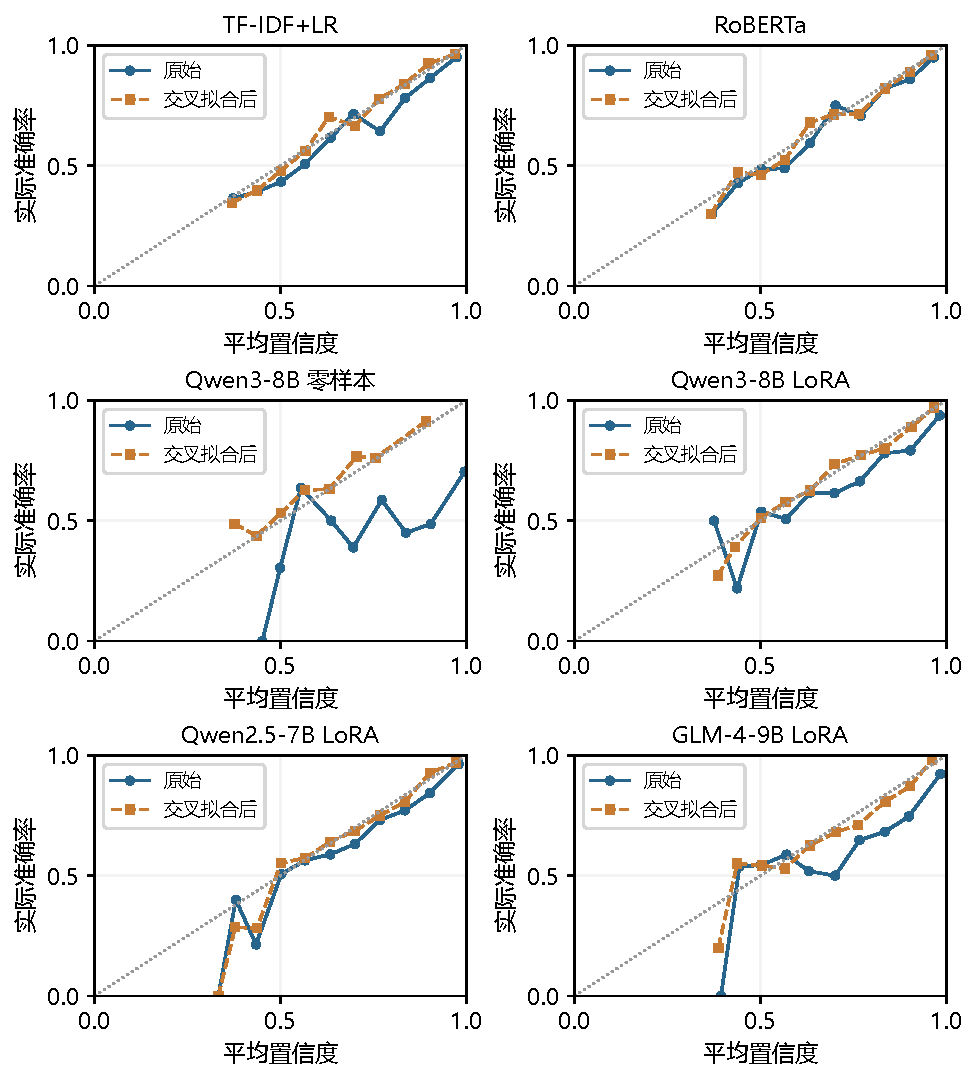
\includegraphics[width=\linewidth,height=0.80\textheight,keepaspectratio]{figures/fig_reliability.pdf}
\caption{可靠性图（对角线表示完美校准，曲线位于对角线下方表示过度自信）}\label{fig:4-2}\end{figure}

结果显示出三个特点：

第一，未经微调的大模型严重过度自信。Qwen3-8B 零样本的平均置信度高达 96.4\%，实际准确率只有 67.1\%，ECE 为 0.294，NLL 为 3.33，在当前截断约定下得到平均温度 T = 9.85；置信度与准确率之间的差距支持过度自信判断，但 NLL 和温度的具体数值需结合存储精度限制解释。

第二，LoRA 微调大幅改善了校准，但大模型仍比 RoBERTa 更加过度自信。三个 LoRA 大模型的 ECE 在 0.035～0.085 之间，平均置信度均高于准确率，最优温度均大于 1；其中 GLM-4-9B 最明显（置信度 90.0\%，准确率 81.9\%）。RoBERTa 的 ECE 为 0.031，是未校准时最低的。这说明训练后的概率仍需要单独评估，与第 2 章区分判别能力和不确定性评估的思路相一致。值得注意的是，在 Brier 分数和 NLL 这两个同时反映判别能力和校准的指标上，Qwen 系列的 LoRA 模型仍优于 RoBERTa。

第三，在当前测试分布内，五折温度交叉拟合降低了 ECE。各模型的 ECE 降到 0.013～0.030，其中 Qwen3-8B LoRA 从 0.061 降到 0.013，是本表 ECE 最低者。对单个样本，正温度不改变其类别 logits 的大小顺序，因此不改变预测类别、准确率和 Macro-F1；这并不意味着跨样本的置信度排序一定不变。本文的选择性预测仍使用原始概率排序，没有把校准后的结果与其混用。

需要特别说明，Qwen3 零样本的 1713 条预测中有 91 条真实类别概率在历史 CSV 中为零。仅将截断下限从 1e-12 改为 1e-8 或 1e-6，NLL 就由 3.3301 变为 2.8408 或 2.5962，平均温度由 9.8543 变为 7.5518 或 6.5507。上述变化是数值敏感性，不是不同模型效果；任何一个截断下限都不能恢复原始 logits。本轮未重新推理，因此保留原表并明确其约定，后续应保存高精度概率或 logits 后再核验零样本 NLL、温度及极端分数并列。Qwen3 LoRA 本次没有零概率，在这些下限下指标不变；不能把零样本敏感性泛化到全部模型。完整结果见 outputs/analysis/probability\_precision.csv。

\FloatBarrier\subsection{选择性预测}

表~\ref{tab:4-9} 和图~\ref{fig:4-3} 给出了各模型的选择性预测结果。

\begin{table}[htbp]
\centering
\begin{minipage}{\textwidth}
\setlength{\tabcolsep}{3pt}
\renewcommand{\arraystretch}{1.16}
\setstretch{1.0}\fontsize{10.5}{13.5}\selectfont
\caption{选择性预测结果（种子 42）}\label{tab:4-9}
\begin{tabular}{>{\raggedright\arraybackslash}p{\dimexpr 0.280000\linewidth-3.920000\tabcolsep\relax}>{\raggedright\arraybackslash}p{\dimexpr 0.100000\linewidth-1.400000\tabcolsep\relax}>{\raggedright\arraybackslash}p{\dimexpr 0.100000\linewidth-1.400000\tabcolsep\relax}>{\raggedright\arraybackslash}p{\dimexpr 0.130000\linewidth-1.820000\tabcolsep\relax}>{\raggedright\arraybackslash}p{\dimexpr 0.130000\linewidth-1.820000\tabcolsep\relax}>{\raggedright\arraybackslash}p{\dimexpr 0.130000\linewidth-1.820000\tabcolsep\relax}>{\raggedright\arraybackslash}p{\dimexpr 0.130000\linewidth-1.820000\tabcolsep\relax}}
\toprule
\textbf{模型} & \textbf{AURC} & \textbf{E-\allowbreak{}AURC} & \textbf{覆盖 50\% 准确率} & \textbf{覆盖 80\% 准确率} & \textbf{覆盖 90\% 准确率} & \textbf{全部作答准确率} \\
\midrule
TF-\allowbreak{}IDF+LR & 0.114 & 0.075 & 0.895 & 0.806 & 0.772 & 0.734 \\
RoBERTa & 0.074 & 0.054 & 0.943 & 0.880 & 0.846 & 0.806 \\
Qwen3-\allowbreak{}8B 零样本 & 0.200 & 0.138 & 0.804 & 0.722 & 0.693 & 0.671 \\
Qwen3-\allowbreak{}8B LoRA & 0.060 & 0.043 & 0.957 & 0.891 & 0.859 & 0.821 \\
Qwen2.5-\allowbreak{}7B LoRA & 0.060 & 0.042 & 0.961 & 0.888 & 0.856 & 0.818 \\
GLM-\allowbreak{}4-\allowbreak{}9B LoRA & 0.062 & 0.045 & 0.954 & 0.882 & 0.849 & 0.819 \\
\bottomrule\end{tabular}
\end{minipage}
\end{table}

\begin{figure}[htbp]\centering
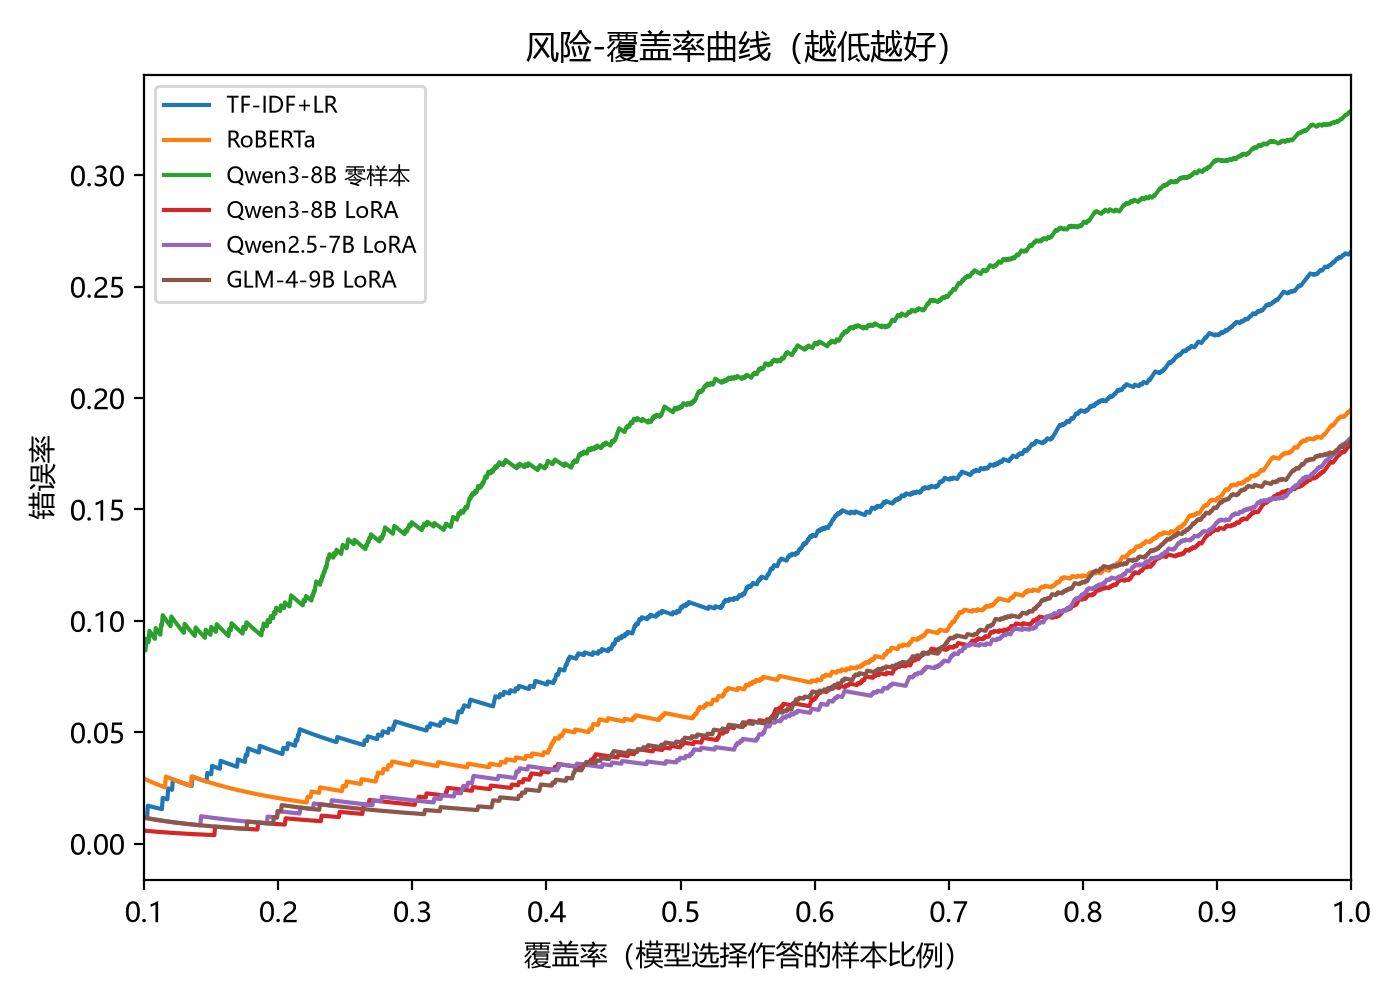
\includegraphics[width=\linewidth,height=0.80\textheight,keepaspectratio]{figures/fig_risk_coverage.png}
\caption{风险-\allowbreak{}覆盖率曲线}\label{fig:4-3}\end{figure}

三个 LoRA 大模型的 AURC 约为 0.060，明显低于 RoBERTa（0.074）和 TF-IDF（0.114）。E-AURC 的排序与之相同，说明大模型的优势不仅来自更高的整体准确率，也来自置信度对对错更好的区分能力。换言之，大模型虽然整体上过度自信，但它``更有把握''的样本确实更可能判断正确。

从应用角度看，若只让 Qwen2.5-7B LoRA 回答置信度最高的 50\% 评论，准确率可达 96.1\%；覆盖 80\% 时准确率仍有 88.8\%。这为部分自动化提供了数据内参考；实际阈值仍须在独立校准集确定，再在新样本上验证，本文未验证部署错误率或实际人工成本。

\FloatBarrier\subsection{消融实验}

为分析训练样本量、LoRA 秩和量化精度对效果的影响，本文以 Qwen3-8B 为对象、固定种子 42 进行了消融实验，结果见表~\ref{tab:4-10} 和图~\ref{fig:4-4}。训练样本量实验中，由于样本较少，训练轮数由 2 轮增加到 3 轮。

\begin{table}[htbp]
\centering
\begin{minipage}{\textwidth}
\setlength{\tabcolsep}{3pt}
\renewcommand{\arraystretch}{1.16}
\setstretch{1.0}\fontsize{10.5}{13.5}\selectfont
\caption{消融实验结果（Qwen3-\allowbreak{}8B，种子 42）}\label{tab:4-10}
\begin{tabular}{>{\raggedright\arraybackslash}p{\dimexpr 0.200000\linewidth-2.000000\tabcolsep\relax}>{\raggedright\arraybackslash}p{\dimexpr 0.200000\linewidth-2.000000\tabcolsep\relax}>{\raggedright\arraybackslash}p{\dimexpr 0.200000\linewidth-2.000000\tabcolsep\relax}>{\raggedright\arraybackslash}p{\dimexpr 0.200000\linewidth-2.000000\tabcolsep\relax}>{\raggedright\arraybackslash}p{\dimexpr 0.200000\linewidth-2.000000\tabcolsep\relax}}
\toprule
\textbf{消融因素} & \textbf{设置} & \textbf{Macro-\allowbreak{}F1} & \textbf{准确率} & \textbf{峰值显存} \\
\midrule
训练样本量 & 0（零样本） & 0.644 & 0.671 & — \\
训练样本量 & 500 & 0.766 & 0.790 & — \\
训练样本量 & 1000 & 0.772 & 0.788 & — \\
训练样本量 & 2000 & 0.770 & 0.790 & — \\
训练样本量 & 4000 & 0.789 & 0.809 & — \\
训练样本量 & 8802（全部） & 0.800 & 0.821 & 18.3 GB \\
LoRA 秩 & r = 4（1091 万参数） & 0.804 & 0.825 & 17.9 GB \\
LoRA 秩 & r = 8（2182 万参数） & 0.809 & 0.828 & 18.1 GB \\
LoRA 秩 & r = 16（4365 万参数） & 0.800 & 0.821 & 18.3 GB \\
LoRA 秩 & r = 32（8729 万参数） & 0.798 & 0.818 & 18.9 GB \\
量化精度 & 16 位（bf16） & 0.800 & 0.821 & 18.3 GB \\
量化精度 & 4 位（QLoRA） & 0.807 & 0.828 & 11.2 GB \\
\bottomrule\end{tabular}
\end{minipage}
\end{table}

\begin{figure}[htbp]\centering
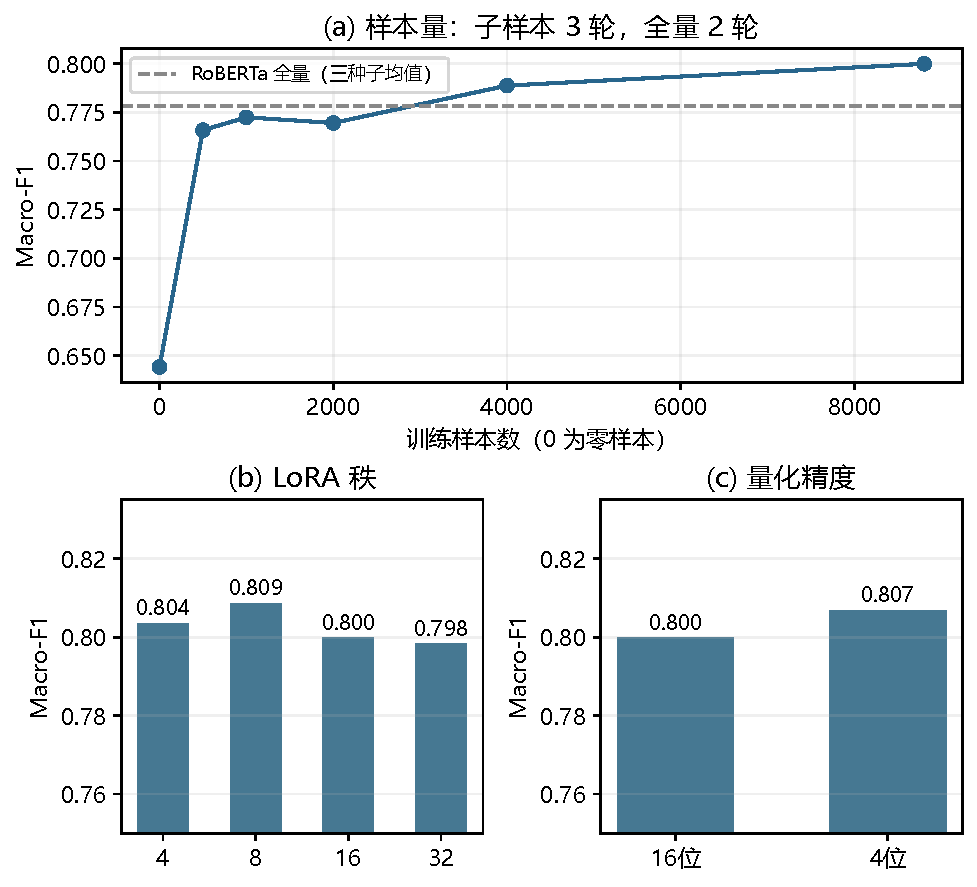
\includegraphics[width=\linewidth,height=0.80\textheight,keepaspectratio]{figures/fig_ablation.pdf}
\caption{Qwen3-\allowbreak{}8B LoRA 消融实验}\label{fig:4-4}\end{figure}

\textbf{训练样本量。} 只用 500 条样本微调，Macro-F1 就从零样本的 0.644 提高到 0.766，接近用全部 8802 条数据训练的 RoBERTa（0.778）。此后继续增加数据，效果提升逐渐放缓：从 500 条增加到 8802 条，数据量增加约 17 倍，Macro-F1 只提高 3.4 个百分点。这说明大模型只需少量标注数据就能适应任务，在标注成本较高的金融场景中有实际意义。

\textbf{LoRA 秩。} 秩从 4 增加到 32，可训练参数增加 8 倍，Macro-F1 却在 0.798～0.809 之间小幅波动，没有随参数增加而提高。考虑到同一模型不同种子之间的标准差约为 0.002～0.007，且每个秩只运行了一次，当前只能描述各秩的单次结果接近；缺少各秩多次重复和等效性检验，不能据此证明各秩等效或任务只需要某个固定更新量。

\textbf{量化精度。} 4-bit 量化将训练峰值显存从 18.3 GB 降到 11.2 GB，降幅约 39\%，而 Macro-F1 没有下降（0.807 对 0.800），代价是训练时间从 38 分钟增加到 44 分钟。这里的显存指标来自框架的峰值已分配内存，不等于整卡实际占用；因此该结果提示较低资源配置的可行性，但不能保证任意 12 GB 显卡及软件环境均可运行，也不能由一次实验证明两种精度等效。

\FloatBarrier\subsection{评估曝光与清洗策略比较}

本文保留了未清洗策略的实验：原始训练文件随机划出 10\% 作为验证集，在其余样本上训练 TF-IDF+LR 和 RoBERTa（3 个种子），再评估原始 eval\_list 的 2020 条记录。原始训练文件中的记录不都参与参数优化，因此区分两种曝光口径：

（1）以原始训练文件（包含后来划出的验证集）为基准，seen\_same / seen\_diff / unseen 为 868 / 229 / 923； （2）只以实际优化训练集为基准，三组为 787 / 202 / 1031。其中 108 条评估记录仅在验证集出现，不在优化训练集出现。验证集参与模型选择，仍属于开发数据曝光，但不能直接称为训练时``背答案''。

表~\ref{tab:4-11} 采用第二种口径，RoBERTa 报告三个种子的平均指标。这里的``训练中未见''包括验证曝光记录，不等于完全独立于模型开发。

\begin{table}[htbp]
\centering
\begin{minipage}{\textwidth}
\setlength{\tabcolsep}{3pt}
\renewcommand{\arraystretch}{1.16}
\setstretch{1.0}\fontsize{10.5}{13.5}\selectfont
\caption{按实际优化训练集曝光分组的评估结果}\label{tab:4-11}
\begin{tabular}{>{\raggedright\arraybackslash}p{\dimexpr 0.300000\linewidth-3.600000\tabcolsep\relax}>{\raggedright\arraybackslash}p{\dimexpr 0.100000\linewidth-1.200000\tabcolsep\relax}>{\raggedright\arraybackslash}p{\dimexpr 0.150000\linewidth-1.800000\tabcolsep\relax}>{\raggedright\arraybackslash}p{\dimexpr 0.150000\linewidth-1.800000\tabcolsep\relax}>{\raggedright\arraybackslash}p{\dimexpr 0.150000\linewidth-1.800000\tabcolsep\relax}>{\raggedright\arraybackslash}p{\dimexpr 0.150000\linewidth-1.800000\tabcolsep\relax}}
\toprule
\textbf{测试子集} & \textbf{样本数} & \textbf{TF-\allowbreak{}IDF+LR 准确率} & \textbf{TF-\allowbreak{}IDF+LR Macro-\allowbreak{}F1} & \textbf{RoBERTa 准确率} & \textbf{RoBERTa Macro-\allowbreak{}F1} \\
\midrule
原始全部评估集 & 2020 & 0.7703 & 0.7547 & 0.7881 & 0.7734 \\
优化训练中见过且含同标签 & 787 & 0.9975 & 0.9974 & 0.9399 & 0.9371 \\
优化训练中见过但仅含不同标签 & 202 & 0.0000 & 0.0000 & 0.1881 & 0.1915 \\
优化训练中未见（含验证曝光） & 1031 & 0.7478 & 0.6767 & 0.7898 & 0.7411 \\
\bottomrule\end{tabular}
\end{minipage}
\end{table}

对实际优化训练中存在相同标签的原句，TF-IDF 的准确率为 99.75\%，RoBERTa 为 93.99\%；在优化训练中仅有不同标签的子集上，两者分别为 0\% 和 18.81\%。这与模型对已曝光文本的记忆相一致，但分组并非随机，样本难度和类别构成也不同，不能用组间差值识别纯泄漏效应。

为与原分析口径对照，原始训练文件意义下的全体评估与 unseen 子集上，TF-IDF 的 Macro-F1 分别为 0.7547 与 0.6733，差约 8.14 个百分点；RoBERTa 分别为 0.7734 与 0.7400，差约 3.34 个百分点。这些是不同样本总体的描述差：unseen 子集积极类占 63.1\%，seen\_same 中仅占 28.1\%，Macro-F1 也不满足按子集比例线性加权。因此不将 8.14 个百分点称为纯泄漏造成的虚高，也不把不同子集中的模型差距变化称为``真实差距被缩小''。

进一步将两种训练策略严格对齐到同样的 845 条共同未曝光文本及相同标签上，TF-IDF 的 Macro-F1 为 0.6543（未清洗训练）和 0.6583（清洗后训练）；RoBERTa 三种子均值为 0.7309 和 0.7392。这一比较没有观察到 F1 点估计下降，但尚未作等效性检验，且同时改变了去重、冲突处理和训练样本构成，只能解释为清洗策略的整体比较。若要估计单独的泄漏因果效应，需要固定测试样本并控制其他处理因素。详细分组和共同样本结果分别见 outputs/analysis/leakage.csv 与 outputs/analysis/leakage\_matched.csv。

\FloatBarrier\subsection{重复记录一致性与噪声情景分析}

原始 FinFE 两个文件中有 5575 个规范化文本出现两次及以上，对每个文本的全部记录作两两配对，共得到 6048 对。文件不提供标注者 ID、独立复标过程或金标准，因此下文描述的是重复记录的一致性，而非已经确认的独立人工复标可靠性。

\begin{table}[htbp]
\centering
\begin{minipage}{\textwidth}
\setlength{\tabcolsep}{3pt}
\renewcommand{\arraystretch}{1.16}
\setstretch{1.0}\fontsize{10.5}{13.5}\selectfont
\caption{重复记录的标签一致性分析}\label{tab:4-12}
\begin{tabular}{>{\raggedright\arraybackslash}p{\dimexpr 0.460000\linewidth-1.840000\tabcolsep\relax}>{\raggedright\arraybackslash}p{\dimexpr 0.540000\linewidth-2.160000\tabcolsep\relax}}
\toprule
\textbf{指标} & \textbf{数值} \\
\midrule
重复文本数 /\allowbreak{} 记录配对数 & 5575 /\allowbreak{} 6048 \\
配对一致率 p\_\allowbreak{}o & 0.8289（文本级 Bootstrap 95\% CI：0.8135～0.8452） \\
随机一致率 p\_\allowbreak{}e,pair（配对两端汇总边际） & 0.3375 \\
机会校正一致性 K\_\allowbreak{}pair（非标准 Cohen $\kappa$） & 0.7417 \\
独立同质对称噪声假设下的情景 q & 0.9081（条件于模型的 Bootstrap 区间：0.8991～0.9175） \\
冲突配对：消极—中性 /\allowbreak{} 中性—积极 /\allowbreak{} 消极—积极 & 475 /\allowbreak{} 374 /\allowbreak{} 186 \\
\bottomrule\end{tabular}
\end{minipage}
\end{table}

一致率以配对数加权，同一文本出现较多次时贡献更多配对；置信区间按文本整组重抽样，保留组内依赖。每个文本固定取前两条记录时，一致率为 0.8196，可见权重口径有一定影响。K\_pair 使用配对两端的汇总边际，与一致率的抽样单位一致；由于没有固定两名标注者，本文不称其为标准 Cohen \(\kappa\)，也不套用双标注者可靠性的等级标签。

在给定真实类别后两次标注独立、同质且均匀错标的假设下，可由 p\_o = q\(^{2}\) + (1 \(-\) q)\(^{2}\)/2 推算 q \(\approx\) 0.9081。该值及区间均条件于上述模型；它们不包含噪声模型可能不成立的不确定性。重复文本平均长度为 18.5 个字符，短于全部文本的 21.1，且清洗后测试集已删除部分冲突记录，故不把该推算当作清洗后测试集的实测准确率上限，也不以模型准确率约 82\% 与记录一致率 82.9\% 的接近宣称模型接近人工水平。

全部 1035 个冲突配对中有 849 个（82.0\%）涉及中性类。这与模型在中性类上较难取得高 F1 的现象相一致，但冲突比例还受类别构成和重复记录选择影响，不能单独证明中性类错误主要由标注噪声造成。

\FloatBarrier\subsection{保形预测}

保形预测（conformal prediction）\cite{ref31,ref32} 输出类别集合。在校准样本与新评估样本可交换、模型及评分规则固定的条件下，它提供 P\{Y \(\in\) C(X)\} \(\ge\) 1 \(-\) \(\alpha\) 的边际覆盖保证；这不是每条预测或任意筛选子集都具有相同正确率的保证。

本文采用分割保形预测，以 s = 1 \(-\) p(真实类) 为非一致性分数，将 1713 条测试记录随机分为 856 条校准和 857 条评估记录；在校准部分取第 \(\lceil\)(n+1)(1\(-\alpha\))\(\rceil\) 个次序统计量 \(\hat q\)，在评估部分输出集合 \{k : 1 \(-\) p\_k \(\le\) \(\hat q\)\}。每次划分不使用评估标签计算阈值；重复 1000 次取平均，仅描述同一批数据内的划分变化，不将其当成 1000 个独立外部测试集。另采用类内分别求 \(\hat q\) 的 Mondrian 方法，其类别条件保证仍要求相应类内交换性。

\begin{table}[htbp]
\centering
\begin{minipage}{\textwidth}
\setlength{\tabcolsep}{3pt}
\renewcommand{\arraystretch}{1.16}
\setstretch{1.0}\fontsize{10.5}{13.5}\selectfont
\caption{保形预测的整体覆盖与集合效率}\label{tab:4-13}
\begin{tabular}{>{\raggedright\arraybackslash}p{\dimexpr 0.320000\linewidth-3.200000\tabcolsep\relax}>{\raggedright\arraybackslash}p{\dimexpr 0.120000\linewidth-1.200000\tabcolsep\relax}>{\raggedright\arraybackslash}p{\dimexpr 0.160000\linewidth-1.600000\tabcolsep\relax}>{\raggedright\arraybackslash}p{\dimexpr 0.200000\linewidth-2.000000\tabcolsep\relax}>{\raggedright\arraybackslash}p{\dimexpr 0.200000\linewidth-2.000000\tabcolsep\relax}}
\toprule
\textbf{模型} & \textbf{方法} & \textbf{覆盖率} & \textbf{平均集合大小} & \textbf{单元素比例} \\
\midrule
TF-\allowbreak{}IDF+LR & 标准 & 0.9008 & 1.580 & 52.88\% \\
TF-\allowbreak{}IDF+LR & 按类别 & 0.9011 & 1.609 & 47.29\% \\
RoBERTa-\allowbreak{}wwm-\allowbreak{}ext & 标准 & 0.9003 & 1.276 & 74.92\% \\
RoBERTa-\allowbreak{}wwm-\allowbreak{}ext & 按类别 & 0.9017 & 1.354 & 65.86\% \\
Qwen3-\allowbreak{}8B 零样本 & 标准 & 0.9012 & 1.907 & 40.82\% \\
Qwen3-\allowbreak{}8B 零样本 & 按类别 & 0.9275 & 2.035 & 10.32\% \\
Qwen3-\allowbreak{}8B LoRA & 标准 & 0.9005 & 1.247 & 77.89\% \\
Qwen3-\allowbreak{}8B LoRA & 按类别 & 0.9012 & 1.296 & 71.11\% \\
Qwen2.5-\allowbreak{}7B LoRA & 标准 & 0.9008 & 1.248 & 77.09\% \\
Qwen2.5-\allowbreak{}7B LoRA & 按类别 & 0.9023 & 1.288 & 72.25\% \\
GLM-\allowbreak{}4-\allowbreak{}9B LoRA & 标准 & 0.9010 & 1.247 & 77.67\% \\
GLM-\allowbreak{}4-\allowbreak{}9B LoRA & 按类别 & 0.9014 & 1.316 & 70.07\% \\
\bottomrule\end{tabular}
\par\vspace{3pt}{\fontsize{10}{12.5}\selectfont 注：目标边际覆盖率 90\%；种子 42 预测，1000 次内部随机划分均值；不是 1000 个独立外部测试。\par}
\end{minipage}
\end{table}

\begin{table}[htbp]
\centering
\begin{minipage}{\textwidth}
\setlength{\tabcolsep}{3pt}
\renewcommand{\arraystretch}{1.16}
\setstretch{1.0}\fontsize{10.5}{13.5}\selectfont
\caption{保形预测的类别条件经验覆盖率}\label{tab:4-14}
\begin{tabular}{>{\raggedright\arraybackslash}p{\dimexpr 0.320000\linewidth-3.200000\tabcolsep\relax}>{\raggedright\arraybackslash}p{\dimexpr 0.140000\linewidth-1.400000\tabcolsep\relax}>{\raggedright\arraybackslash}p{\dimexpr 0.180000\linewidth-1.800000\tabcolsep\relax}>{\raggedright\arraybackslash}p{\dimexpr 0.180000\linewidth-1.800000\tabcolsep\relax}>{\raggedright\arraybackslash}p{\dimexpr 0.180000\linewidth-1.800000\tabcolsep\relax}}
\toprule
\textbf{模型} & \textbf{方法} & \textbf{消极覆盖率} & \textbf{中性覆盖率} & \textbf{积极覆盖率} \\
\midrule
TF-\allowbreak{}IDF+LR & 标准 & 0.9080 & 0.7828 & 0.9601 \\
TF-\allowbreak{}IDF+LR & 按类别 & 0.9014 & 0.9011 & 0.9009 \\
RoBERTa-\allowbreak{}wwm-\allowbreak{}ext & 标准 & 0.9200 & 0.7620 & 0.9636 \\
RoBERTa-\allowbreak{}wwm-\allowbreak{}ext & 按类别 & 0.9022 & 0.9023 & 0.9011 \\
Qwen3-\allowbreak{}8B 零样本 & 标准 & 0.9977 & 0.7685 & 0.9180 \\
Qwen3-\allowbreak{}8B 零样本 & 按类别 & 0.9032 & 1.0000 & 0.9024 \\
Qwen3-\allowbreak{}8B LoRA & 标准 & 0.9069 & 0.7761 & 0.9641 \\
Qwen3-\allowbreak{}8B LoRA & 按类别 & 0.9012 & 0.9030 & 0.9000 \\
Qwen2.5-\allowbreak{}7B LoRA & 标准 & 0.9321 & 0.7576 & 0.9600 \\
Qwen2.5-\allowbreak{}7B LoRA & 按类别 & 0.9022 & 0.9037 & 0.9015 \\
GLM-\allowbreak{}4-\allowbreak{}9B LoRA & 标准 & 0.8961 & 0.8042 & 0.9559 \\
GLM-\allowbreak{}4-\allowbreak{}9B LoRA & 按类别 & 0.9027 & 0.9016 & 0.9006 \\
\bottomrule\end{tabular}
\par\vspace{3pt}{\fontsize{10}{12.5}\selectfont 注：沿用表 4-\allowbreak{}13 的同一批划分；按类别方法分别校准，但不由此推出单元素子集正确率保证。\par}
\end{minipage}
\end{table}

标准方法下，各模型的平均整体覆盖率约为 90\%，与名义目标相近；有限评估样本下，某一次划分的经验覆盖率仍可能低于 90\%。这些均值支持当前数据内的覆盖表现，但不能由有限次实验``证明''面向所有未来分布的保证。目标 95\% 的结果及各次划分覆盖率的经验分位数见 outputs/analysis/conformal.csv。

LoRA 模型的标准预测集合平均大小约为 1.25，单元素集合比例约为 77\%～78\%，比 TF-IDF 和零样本 Qwen3 更精简。为避免把边际覆盖与单元素答案正确率混淆，表~\ref{tab:4-15} 单独报告单元素子集上的经验准确率。

\begin{table}[htbp]
\centering
\begin{minipage}{\textwidth}
\setlength{\tabcolsep}{3pt}
\renewcommand{\arraystretch}{1.16}
\setstretch{1.0}\fontsize{10.5}{13.5}\selectfont
\caption{标准保形预测的单元素集合表现（目标边际覆盖率 90\%）}\label{tab:4-15}
\begin{tabular}{>{\raggedright\arraybackslash}p{\dimexpr 0.400000\linewidth-2.400000\tabcolsep\relax}>{\raggedright\arraybackslash}p{\dimexpr 0.300000\linewidth-1.800000\tabcolsep\relax}>{\raggedright\arraybackslash}p{\dimexpr 0.300000\linewidth-1.800000\tabcolsep\relax}}
\toprule
\textbf{模型} & \textbf{单元素集合比例} & \textbf{单元素集合内准确率} \\
\midrule
Qwen3-\allowbreak{}8B LoRA & 77.89\% & 89.25\% \\
Qwen2.5-\allowbreak{}7B LoRA & 77.09\% & 89.31\% \\
GLM-\allowbreak{}4-\allowbreak{}9B LoRA & 77.67\% & 88.75\% \\
\bottomrule\end{tabular}
\end{minipage}
\end{table}

准确率为 1000 次划分中单元素预测的正确总数除以单元素预测总数，重复出现的样本不视为独立观测来构造额外置信区间。三个 LoRA 模型的单元素准确率仅为 88.7\%～89.3\%，因此不能说约 78\% 的评论获得了``有 90\% 保证的唯一答案''。集合大小、整体覆盖率和单元素正确率应分别报告。

表~\ref{tab:4-14} 显示，标准方法下中性类覆盖率约为 0.76～0.80；对三个 LoRA 模型，按类别校准后各类平均经验覆盖率接近 0.90，平均集合大小增加约 0.04～0.07，单元素比例相应下降。这说明保护较难类别需要付出预测集合变大的代价，不等于消除了模型对中性类的所有错误。

Qwen3 零样本在按类别校准时出现明显过度覆盖，目标 90\% 时平均覆盖率约为 0.9275，中性类接近 1。历史概率存在精度损失和大量并列分数，不能将这些并列全部归因于模型固有行为。保形预测的边际下界不要求模型本身概率校准良好，但集合效率及过度覆盖程度会受评分质量和数值精度影响。

\FloatBarrier\subsection{真实预测的错误结构与案例}

\subsubsection{类条件混淆与模型互补性}

图~\ref{fig:4-5} 的三组预测与同一 1713 条测试文本和标签逐行对齐；混淆矩阵按观测类别归一化，单元格同时保留样本数。观测标签不是经本研究重新核定的金标准。

\begin{figure}[htbp]\centering
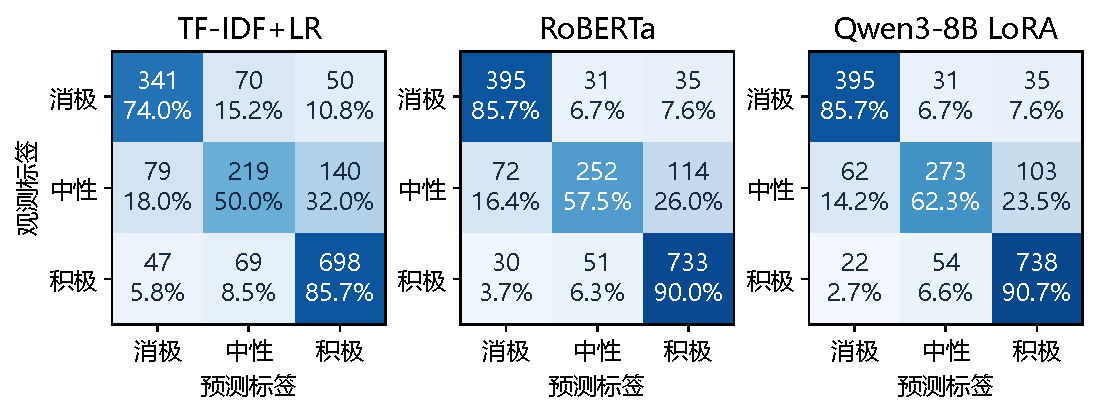
\includegraphics[width=\linewidth,height=0.80\textheight,keepaspectratio]{figures/fig_confusion.pdf}
\caption{种子 42 的混淆矩阵（计数与行内比例）}\label{fig:4-5}\end{figure}

\begin{table}[htbp]
\centering
\begin{minipage}{\textwidth}
\setlength{\tabcolsep}{3pt}
\renewcommand{\arraystretch}{1.16}
\setstretch{1.0}\fontsize{10.5}{13.5}\selectfont
\caption{种子 42 的类别指标}\label{tab:4-16}
\begin{tabular}{>{\raggedright\arraybackslash}p{\dimexpr 0.290000\linewidth-3.480000\tabcolsep\relax}>{\raggedright\arraybackslash}p{\dimexpr 0.130000\linewidth-1.560000\tabcolsep\relax}>{\raggedright\arraybackslash}p{\dimexpr 0.130000\linewidth-1.560000\tabcolsep\relax}>{\raggedright\arraybackslash}p{\dimexpr 0.150000\linewidth-1.800000\tabcolsep\relax}>{\raggedright\arraybackslash}p{\dimexpr 0.150000\linewidth-1.800000\tabcolsep\relax}>{\raggedright\arraybackslash}p{\dimexpr 0.150000\linewidth-1.800000\tabcolsep\relax}}
\toprule
\textbf{模型} & \textbf{观测类别} & \textbf{样本数} & \textbf{精确率} & \textbf{召回率} & \textbf{F1} \\
\midrule
TF-\allowbreak{}IDF+LR & 消极 & 461 & 0.730 & 0.740 & 0.735 \\
TF-\allowbreak{}IDF+LR & 中性 & 438 & 0.612 & 0.500 & 0.550 \\
TF-\allowbreak{}IDF+LR & 积极 & 814 & 0.786 & 0.857 & 0.820 \\
RoBERTa & 消极 & 461 & 0.795 & 0.857 & 0.825 \\
RoBERTa & 中性 & 438 & 0.754 & 0.575 & 0.653 \\
RoBERTa & 积极 & 814 & 0.831 & 0.900 & 0.864 \\
Qwen3-\allowbreak{}8B LoRA & 消极 & 461 & 0.825 & 0.857 & 0.840 \\
Qwen3-\allowbreak{}8B LoRA & 中性 & 438 & 0.763 & 0.623 & 0.686 \\
Qwen3-\allowbreak{}8B LoRA & 积极 & 814 & 0.842 & 0.907 & 0.873 \\
\bottomrule\end{tabular}
\par\vspace{3pt}{\fontsize{10}{12.5}\selectfont 注：所有指标直接由保存的离散预测计算；与表 4-\allowbreak{}2 的多种子均值口径不同。三个模型均以同一观测标签为参照。\par}
\end{minipage}
\end{table}

TF-IDF+LR、RoBERTa、Qwen3 LoRA 分别错误 455、333、307 条，其中涉及中性标签的错误分别为 358、268、250 条，占各自错误的 78.7\%、80.5\%、81.4\%。这里``涉及中性''指观测或预测为中性；不能把它误读为``81.4\% 的中性样本分类错误''。

Qwen3 的中性召回率为 273/438=62.3\%，高于 RoBERTa 的 252/438=57.5\%，但仍低于其消极召回率 85.7\% 与积极召回率 90.7\%。Qwen3 将 103 条中性样本判为积极、62 条判为消极，说明总体增益没有消除中性边界问题。两个模型消极行的汇总计数完全相同，不表示逐条预测也相同。

逐条配对后，Qwen3 修正了 RoBERTa 的 123 条错误，同时在 RoBERTa 正确的样本上新增 97 条错误，两者共同错误 210 条。净少错 26 条并不意味着在所有文本上单向改进；这些计数是第 4.2 节统计比较的可解释补充，而不是新的显著性证明。

\subsubsection{固定规则抽取的真实案例}

表~\ref{tab:4-17} 展示第 3.7.5 节固定抽样的六条案例，完整 12 条核读材料另存 error\_cases.csv。置信度为未温度缩放的最大类别概率，按历史文件精度保留。

\begin{table}[htbp]
\centering
\begin{minipage}{\textwidth}
\setlength{\tabcolsep}{3pt}
\renewcommand{\arraystretch}{1.16}
\setstretch{1.0}\fontsize{10.5}{13.5}\selectfont
\caption{六种误分类方向的固定抽样案例}\label{tab:4-17}
\begin{tabular}{>{\raggedright\arraybackslash}p{\dimexpr 0.080000\linewidth-0.640000\tabcolsep\relax}>{\raggedright\arraybackslash}p{\dimexpr 0.180000\linewidth-1.440000\tabcolsep\relax}>{\raggedright\arraybackslash}p{\dimexpr 0.610000\linewidth-4.880000\tabcolsep\relax}>{\raggedright\arraybackslash}p{\dimexpr 0.130000\linewidth-1.040000\tabcolsep\relax}}
\toprule
\textbf{行号} & \textbf{观测$\to$Qwen3预测} & \textbf{原始文本} & \textbf{原始置信度} \\
\midrule
300 & 消极$\to$中性 & 人民文学出版社、中华书局、商务印书馆、中华大百科,人民音乐出版社。唉可惜都不是资本喜欢的。 & 0.794 \\
324 & 消极$\to$积极 & 今天亏了4千3;不错不错;晚上吃炖好的犒劳一下自己 & 0.414 \\
921 & 中性$\to$消极 & 我就纳闷是哪个NT老师说35再买的 & 0.556 \\
1616 & 中性$\to$积极 & 这跟江铜差了7元,早知道多买点江铜了 & 0.934 \\
29 & 积极$\to$消极 & 13.15到13.50为最佳位置,工厂放假生产处与半停产状态,现在买进被套后,舂节后解放 & 0.695 \\
897 & 积极$\to$中性 & 感谢夏利.感谢张婷! & 0.559 \\
\bottomrule\end{tabular}
\par\vspace{3pt}{\fontsize{10}{12.5}\selectfont 注：行号从清洗后 test.jsonl 的第一条数据起计为 1；预测 CSV 另有一行表头。原文保留已有错字、简称及标点，箭头左侧是观测标签，不表示本文认可其为唯一正确判断。\par}
\end{minipage}
\end{table}

\textbf{局部正负线索相互冲突。} 第 324 行同时出现``亏了''与``不错不错''，存在反讽或自我宽慰的可能；Qwen3 与 RoBERTa 均判积极，而 TF-IDF 判消极。第 29 行同时有``半停产''\,``被套''和``春节后解放''的预期表达（原文为``舂节''），Qwen3 判消极，另两模型判积极。这两例说明不同模型会作出不同判断，但没有归因实验，不能声称已证明它们具体依赖了哪个词。

\textbf{观测标签与文本中的态度边界可能不一致。} 第 921 行带有``纳闷''等不满表达，观测为中性，Qwen3 判消极；另两模型为中性。第 1616 行既有价格比较，也有``早知道多买点''的反事实表达，三个模型均判积极而观测为中性，其中 Qwen3 置信度达 0.934。高置信度与模型间一致并不自动证明标签有误，这些例子更适合作为后续独立复标候选。

\textbf{短文本中的评价对象与金融语境不足。} 第 300 行列举出版社后说``唉可惜''，三个模型均判中性而观测为消极。第 897 行的``感谢''表达在缺少上下文时可能难以区分真诚赞许与其他语用，Qwen3 判中性，另两模型判积极。本文只指出可观察的文本特征，不把可能解释写成已验证机制。

以上案例按误分类方向分层，不能代表全部错误的语言类型分布，更不能计算``反讽导致多少错误''。它们与混淆矩阵共同支持的较弱结论是：中性边界、混合态度及上下文不足值得优先复核；不能由个案推出模型知识不足或标注噪声是主要原因。

\FloatBarrier\subsection{本章小结}

围绕 RQ1，LoRA 模型在本划分的三个种子中取得较高点估计，但单次配对检验经多重比较调整后不足以确证相对 RoBERTa 的稳定优势。数据曝光和清洗分析进一步说明，比较分数之前必须统一样本和处理口径。

围绕 RQ2，数据内温度交叉拟合改善了 ECE，高置信度筛选改善了子集准确率，保形方法得到接近名义目标的平均整体覆盖；三者分别回答不同问题，均不能替代独立部署验证。

围绕 RQ3，单次消融支持部分低资源配置的可行性，错误分析揭示中性类仍是主要混淆边界。概率存储精度、非独立复标、样本构成变化和缺少外部测试共同限定了本文结论的外推范围。
